\section{Çerçevenin Yapısı, Bileşenler ve Mimari Tasarım}

\indent \textbf{Projenin başlangıcında}, Türk televizyon dizileriyle ilgili verileri elde etmek için web kazıma (web scraping) yöntemi kullanıldı ve bu veriler Wikipedia'dan çekildi. Ardından, elde edilen dizi bilgileriyle ilgili özel sayfalara gidilerek belirli bilgiler toplandı. Bu bilgiler arasında dizi adı, türü, senarist, yönetmen, başrol oyuncuları, bölüm sayısı gibi detaylar bulunmaktaydı. Ayrıca yapımcı, çekim mekanı, gösterim süresi, yayın tarihi gibi veriler de elde edildi. Bu bilgiler arasında sosyal medya adresleri, yapımcı şirketler ve hangi kanal ya da platformda yayınlandığı gibi detaylar da yer aldı. \\

\indent \textbf{İkinci aşamada}, elde edilen veri setinde eksik olan bilgilerin tamamlanması için Google Sheets gibi bir çevrimiçi tablo platformuna yüklendi. Ekip üyeleri eksik olan verileri el ile girdi. Ardından, Python kullanılarak satırlarda bulunan parantez içindeki ifadeler temizlendi ve gereksiz noktalama işaretleri düzeltildi. \\

\indent \textbf{Üçüncü aşamada}, veri seti üzerinde keşifsel veri analizi yapıldı. Bu analizde, veri setinde en sık geçen değerler belirlendi. Veri analizi sonucunda, elde edilen verilerle ilgili özelliklerin belirlenmesine yönelik fikirler oluşturuldu. \\

\indent \textbf{Dördüncü aşamada} ise özellik çıkarma işlemi gerçekleştirildi. Bu süreçte, veri setinden çeşitli özellikler çıkarıldı ve bu özelliklerin incelenerek hangi bilgilerin daha anlamlı olduğu belirlendi. Veri setinden aşağıdaki özellikler çıkarıldı. \\

\indent \textbf{Beşinci aşamada} model eğitimi sürecinde adımlar şu şekilde gerçekleşti:

\begin{enumerate}
\item \textbf{SelectKBest Yöntemiyle Optimum Özellik Seçimi:} İlk olarak, veri setindeki en önemli özelliklerin belirlenmesi için SelectKBest yöntemi kullanıldı. Bu yöntem, ANOVA F-değeri metoduyla özelliklerin hedef değişkenle ilişkisini değerlendirir. Eğer özellikler sayısal ise, her bir özelliğin hedef değişkenle ilişkisini ifade eden ANOVA F-değerleri hesaplandı. Bu değerler, özelliğin hedef değişkeni ne kadar iyi açıkladığını ölçer.

\item \textbf{Optimum Hiperparametrelerin Belirlenmesi:} Optimum özellik sayısını belirledikten sonra, modelin hiperparametrelerini belirlemek için Optuna gibi bir araç kullanıldı. Optuna, modellerin performansını artırmak için hiperparametre araması yapar. Bayesian Optimization yöntemini kullanarak, model için en iyi parametre setini belirlemek için rastgele parametre kombinasyonları denenir.

\item \textbf{Modelin Oluşturulması ve Kalibrasyonu:} Model oluşturulduktan sonra, modelin çıktılarının daha doğru olması için kalibrasyon işlemi yapıldı. Bu aşamada, "sigmoid" ve "isotonic" gibi kalibrasyon yöntemleri kullanıldı. Sigmoid yöntemi, modelin olasılık tahminlerini sigmoid fonksiyonuyla düzenlerken; isotonic yöntemi ise monoton artış gösteren bir fonksiyonla modelin çıktılarını düzenler.

\item \textbf{HuggingFace Platformu Üzerinden Canlıya Alma:} Son olarak, kalibre edilmiş modeller HuggingFace platformu üzerinde kullanıma hazır hale getirildi. Bu platform, NLP (Doğal Dil İşleme) ve makine öğrenimi modellerini paylaşmak, kullanmak ve dağıtmak için kullanılır.
\end{enumerate}

\begin{figure}[h]
  \centering
  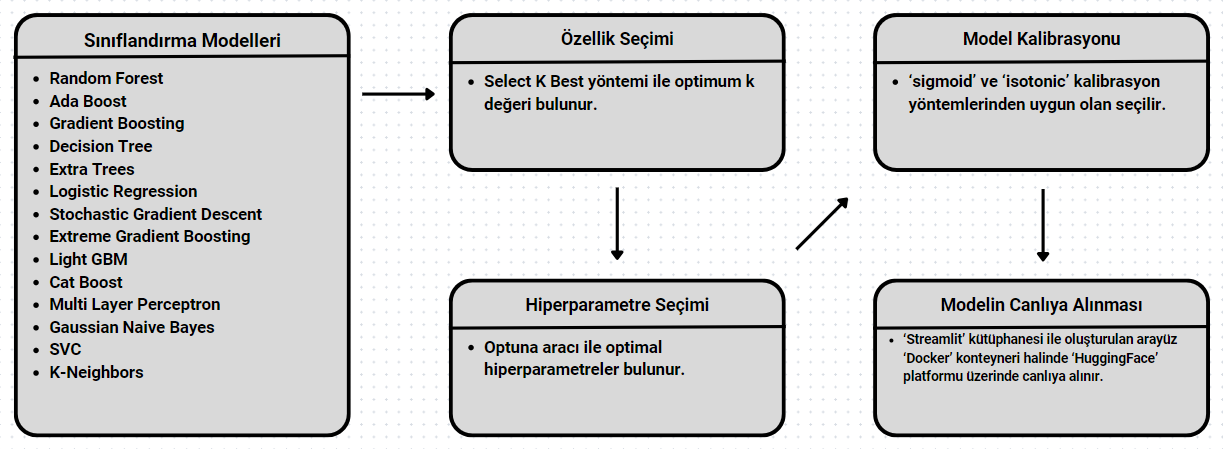
\includegraphics[width=1.0\textwidth]{cerceve.png}
  \caption{Yazılım çerçevesi.}
  \label{fig:ornek_resim}
\end{figure}

\newpage

\begin{table}[h]
\caption{Veri setinden çıkarılan özellikler.}
\label{}
\centering
{\normalsize\renewcommand{\arraystretch}{1.5}
{\resizebox*{\linewidth}{!}{%
\begin{tabular}{|c|c|}
\hline
\textbf{Özellik Adı}                                            & \textbf{Özellik Açıklaması}                                                                                                      \\ \hline
Tarih                                                  & Dizinin çekildiği yıl.                                                                                                  \\ \hline
Dizi adı uzunluğu                                      & Dizi adının uzunluğu.                                                                                                   \\ \hline
Dizi adındaki kelime sayısı                            & Dizi adındaki toplam kelime sayısı.                                                                                     \\ \hline
Dizi adında bağlaç                                     & Dizi adındaki bağlaç sayısı.                                                                                            \\ \hline
Dizi adında yer ismi                                   & Dizi adındaki yer ismi bulunuyor mu ?                                                                                   \\ \hline
Dizi adında özel isim                                  & Dizi adındaki özel isim bulunuyor mu ?                                                                                  \\ \hline
Dizinin türü                                           & Dizi Aile, Aksiyon, Aşk, Bilim Kurgu, Dram, Gençlik, Gerilim, Komedi, Polisiye, Romantik ve Tarihi türlerine sahip mi ? \\ \hline
Dizinin yayınlandığı kanal                             & Dizi TRT 1, Kanal D, atv, Star TV, Show TV, FOX, Samanyolu TV, TV8 kanallarında yayınlanıyor mu ?                       \\ \hline
Çekim yeri                                             & Dizi Türkiyede mi Yurtdışında mı çekilmiş ?                                                                             \\ \hline
Uyarlama                                               & Dizi bir uyarlama mı ?                                                                                                  \\ \hline
Başrol sayısı                                          & Dizideki başrol sayısı.                                                                                                 \\ \hline
Kanal fiyatı                                           & Dizinin yayınlandığı kanal ücretli mi ücretsiz mi ?                                                                     \\ \hline
Yayınlandığı gün                                       & Dizinin yayınlandığı gün.                                                                                               \\ \hline
Yaz dizisi                                             & Temmuz veya Ağustos ayında mı yayınlanmış ?                                                                             \\ \hline
Gösterim süresi                                        & Dizinin bir bölümünün ortalama süresi.                                                                                  \\ \hline
Ödüllü                                                 & Dizi Altın Kelebek ödülü almış mı ?                                                                                     \\ \hline
Senaristlerin yazdığı ortalama dizi sayısı             & Senaristlerin o diziden önce yazdığı ortalama dizi sayısı.                                                              \\ \hline
Ödüllü senarist sayısı                                 & Dizideki ödüllü senarist sayısı.                                                                                        \\ \hline
Senaristlerin aldığı ortalama ödül sayısı              & Senaristlerin aldığı ortalama ödül sayısı.                                                                              \\ \hline
Başrollerin oynadığı ortalama dizi sayısı              & Dizideki başrollerin o diziden önce oynadığı ortalama dizi sayısı.                                                      \\ \hline
Ödüllü başrol sayısı                                   & Dizideki ödüllü başrol sayısı.                                                                                          \\ \hline
Başrollerin aldığı ortalama ödül sayısı                & Başrollerin aldığı ortalama ödül sayısı.                                                                                \\ \hline
Yönetmenlerin yönettiği ortalama dizi sayısı           & Yönetmenlerin o diziden önce yönettiği ortalama dizi sayısı.                                                            \\ \hline
Ödüllü yönetmen sayısı                                 & Dizideki ödüllü yönetmen sayısı.                                                                                        \\ \hline
Yönetmenlerin aldığı ortalama ödül sayısı              & Yönetmenlerin aldığı ortalama ödül sayısı.                                                                              \\ \hline
Görüntü yönetmenlerinin ortalama yönettiği dizi sayısı & Görüntü yönetmenlerinin o diziden önce yönettiği dizi sayısı.                                                           \\ \hline
Bestecilerin bestelediği ortalama dizi sayısı          & Bestecilerin o diziden önce bestelediği ortalama dizi sayısı.                                                           \\ \hline
Yapım şirketlerinin yaptığı ortalama dizi sayısı       & Yapım şirketlerinin o diziden önce yaptıkları ortalama dizi sayısı.                                                     \\ \hline
Sosyal medya hesapları                                 & iziler Youtube, Facebook, Twitter ve Instagram hesabına sahip mi ?                                                      \\ \hline
\end{tabular}%
}}}
\end{table}